\chapter{Introduction}\label{chap:introduction}

Quantum computers are changing the world of online security. This memoire looks at two main things: how quantum computers can break current security methods, and what we can do to stay secure in the future.

Our online world relies on security systems (cryptography) that are designed to be too hard for regular computers to crack. But quantum computers are different. They are much more powerful for certain tasks and can break many of these security systems.

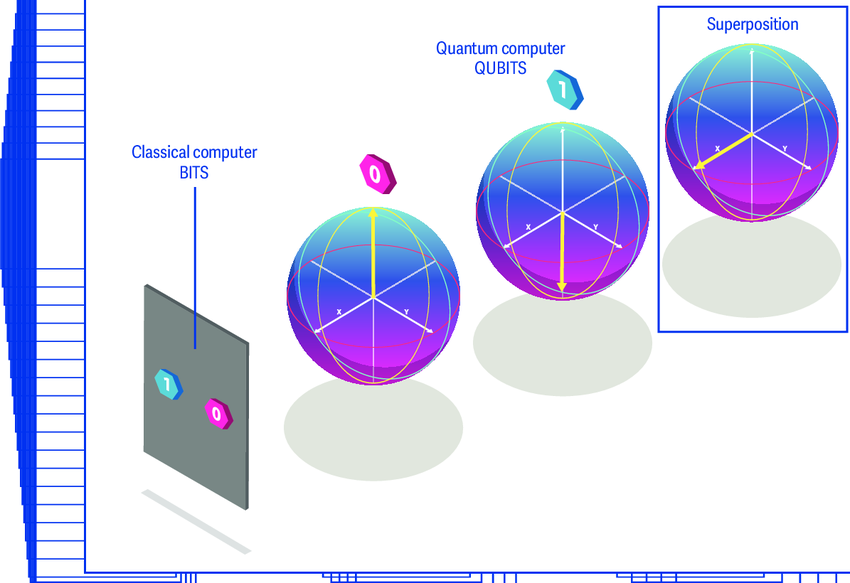
\includegraphics[width=0.8\textwidth]{01_Introduction/quantum_vs_classical}

This quantum threat is a big deal because:
\begin{itemize}
    \item Our current online security might not work against quantum computers.
    \item We urgently need to find new security methods that can resist quantum computers.
    \item Quantum technology itself might also offer new ways to keep things secure.
\end{itemize}

\section{Structure of this Memoire}

This paper is organized chapter by chapter:
\begin{itemize}
    \item \textbf{Chapter 2: Basics of Quantum Computing} --- Explains the core ideas of quantum computing
    \item \textbf{Chapter 3: Regular vs. Quantum Computing} --- Compares regular and quantum computers and why this matters for security
    \item \textbf{Chapter 4: How Current Security Works} --- Reviews the security methods we use today and how they are supposed to be secure
    \item \textbf{Chapter 5: Quantum Threats to Security} --- Explains exactly how quantum computers can break current security systems
    \item \textbf{Chapter 6: Making the Change} --- Looks at the challenges of switching to new, quantum-resistant security systems
    \item \textbf{Chapter 7: New Security Methods} --- Explores security solutions that should work even against quantum computers
    \item \textbf{Chapter 8: What's Next?} --- Considers future developments and trends in this area \parencite{preskill2018quantum}
    \item \textbf{Chapter 9: Impact on Society} --- Discusses the wider effects of these changes beyond just technology
\end{itemize}